\documentclass[10pt,a4paper]{article}

\usepackage{fontspec}
\usepackage[utf8]{inputenc}
\usepackage[italian]{babel}
\usepackage{graphicx}
\usepackage{geometry}
\usepackage{titlesec}
\usepackage{lmodern}
\usepackage{xcolor}
\usepackage{setspace}
\usepackage{titling}
\usepackage{fancyhdr}
\usepackage{float}
\usepackage{minted}
\usepackage{wrapfig}
\usepackage[hidelinks]{hyperref}
\usepackage{tabularx}
\usepackage{listings}
\usepackage{enumitem}


\hypersetup{
    colorlinks,
    citecolor=black,
    filecolor=black,
    linkcolor=black,
    urlcolor=black
}

% riduzione interlinea itemize
\setlist[itemize]{itemsep=2pt, topsep=2pt}

% Definizione di alcuni colori
\definecolor{unipdred}{RGB}{140,0,18}
\definecolor{dunkelblau}{RGB}{0,0,150}
\definecolor{gruen}{RGB}{34,139,34}
\definecolor{lila}{RGB}{128,0,128}

% Small caps + colore per intestazioni
\newcommand{\intestazione}[1]{\textcolor{unipdred}{\textsc{#1}}}

%definizione del package listing per rappresentare il codice sql in maniera corretta
\lstset{
    language=SQL,
    sensitive=false,         
    basicstyle=\ttfamily\small,
    keywordstyle=\color{dunkelblau}\bfseries,
    commentstyle=\color{gruen},
    stringstyle=\color{lila},
    numbers=left,
    numberstyle=\tiny\color{gray},
    breaklines=true,
    showstringspaces=false,
    frame=single
}

\begin{document}
\setmainfont{Arial}
\pagestyle{fancy}
\fancyhead{} % clear all header fields
\fancyfoot{}
\fancyfoot[LE,RO]{\thepage}
\titlespacing*{\section}{0pt}{1ex}{0.5ex}
\titlespacing*{\subsection}{0pt}{0.8ex}{0.4ex}
\titlespacing*{\subsubsection}{0pt}{0.6ex}{0.3ex}
\renewcommand{\arraystretch}{0.9}
\setlength{\tabcolsep}{4pt}

\begin{titlepage}
    \centering

    % Logo
    
\includegraphics[width=0.8\textwidth]{unipd_logo.png} \\[1cm]

    % Intestazioni Università
   % \\[0.2cm]
    {\large \textsc{Dipartimento di Matematica}}\\[0.25cm]
    {\large Laurea Triennale in Informatica}\\[0.25cm]
    {\large Anno Accademico 2025/2026}\\[2.5cm]
    {\LARGE \textsc{Progetto di Basi di Dati}}\\[0.5cm]

    % Riga orizzontale superiore
    \noindent\rule{\textwidth}{0.4pt}\\[0.8cm]

    % Titolo centrale
    {\Huge\bfseries
    Noleggio Auto\\[0.8cm]
    }

    % Riga orizzontale inferiore
    \noindent\rule{\textwidth}{0.4pt}\\[0.8cm]

    % Autori in fondo
    {\LARGE Samuele Gobbi, Gianluca Brotto}
    
\end{titlepage}

%\newpage

\tableofcontents

\newpage

\section{Abstract}
Il progetto sviluppa una base di dati per la gestione di un'azienda di noleggio veicoli organizzata tramite filiali.\\
L'obiettivo del sistema è fornire supporto alla gestione operativa ed economica dell'azienda, organizzando in modo strutturato le informazioni relative ai veicoli, ai clienti, ai contratti, ai pagamenti, alle coperture assicurative e ai vari interventi di manutenzione.\\
La base di dati è organizzata attorno al processo di noleggio: un cliente stipula un contratto presso una filiale di riferimento per l'utilizzo di un determinato veicolo in un intervallo temporale definito. Ad ogni contratto possono essere associate una o più coperture assicurative e uno o più pagamenti, così da consentire il controllo del saldo e dei vari noleggi.\\
Il sistema permette di memorizzare lo stato attuale dei veicoli, distinguendo tra mezzi disponibili, noleggiati e in manutenzione: ogni veicolo noleggiato deve avere un contratto associato a esso, mentre un veicolo in stato di manutenzione deve
avere una manutenzione attiva.\\
Questo sistema aiuta a memorizzare le informazioni in modo efficiente e organizzato, rendendo più facile trovare e analizzare i dati.\\
In questo modo, l'azienda può gestire meglio i suoi veicoli, controllare i contratti e i pagamenti, e prendere decisioni più adeguate.

\section{Analisi dei requisiti} \label{analisirequisiti}
Questa sezione riassume i requisiti a cui deve sottostare la base di dati.

%*************VEICOLI*******************
\noindent
\textbf{Veicolo}: ogni veicolo è identificato da una targa univoca e contiene le seguenti informazioni: 
\begin{itemize}
    \item La \textbf{Targa} che distingue in modo univoco ogni veicolo.
    \item La \textbf{Potenza} espressa in kW.
    \item  L'\textbf{Anno Immatricolazione}.
    \item Il \textbf{Tipo di Alimentazione}.
    \item Il suo \textbf{Stato}, un veicolo può essere in uno stato di \textit{noleggio} se ha un contratto attualmente attivo, in uno stato di \textit{manutenzione} se ha una manutenzione in corso, oppure \textit{disponibile}.
\end{itemize}
\noindent
I Veicoli si distinguono in \textbf{Automobili}, \textbf{Furgoni} e \textbf{Moto}.\\
\textbf{Automobile}. Oltre alle informazioni generali, vengono memorizzati ulteriori dati:
\begin{itemize}
    \item La \textbf{Tipologia}.
    \item Il \textbf{Numero porte}.
\end{itemize}
\textbf{Furgoni}. Oltre alle informazioni generali, vengono memorizzati ulteriori dati:
\begin{itemize}
    \item Il \textbf{Volume}.
    \item La \textbf{Portata}.
\end{itemize}
\textbf{Moto}. Oltre alle informazioni generali, vengono memorizzati ulteriori dati:
\begin{itemize}
    \item La \textbf{Tipologia}.
\end{itemize}
\\
\noindent
I \textbf{Clienti} che stipulano i contratti possiedono i seguenti attributi:
\begin{itemize}
    \item L'\textbf{IdCliente} che permette di identificare in modo univoco il cliente.
    \item L'\textbf{Indirizzo} di residenza, costituito da: \textit{Citta}, \textit{Via}, \textit{Numero}, \textit{cap}.
    \item  Il numero di \textbf{Telefono}.
    \item L'\textbf{Email}.\\
\end{itemize}
\noindent
I Clienti si distinguono in \textbf{Privati} e \textbf{Aziende}.\\
\textbf{Privati}. Oltre alle informazioni generali, vengono memorizzati ulteriori dati:
\begin{itemize}
    \item Il \textbf{Codice fiscale} che permette di identificare ogni cliente privato in modo univoco.
    \item Il \textbf{Nome}.
    \item Il \textbf{Cognome}.
\end{itemize}
\textbf{Azienda}. Oltre alle informazioni generali, vengono memorizzati ulteriori dati:
\begin{itemize}
    \item La \textbf{Partita iva} che permette di identificare ogni azienda in modo univoco.
    \item La \textbf{Ragione Sociale}.
\end{itemize}
\noindent
\textbf{Filiale}: viene identificata da un identificativo univoco e contiene le seguenti informazioni: 
\begin{itemize}
    \item L'\textbf{IdFiliale} che distingue in modo univoco ogni veicolo.
    \item L'\textbf{Indirizzo} in cui è situata la filiale, costituito da: \textit{Citta}, \textit{Via}, \textit{Numero}, \textit{cap}.
    \item  Il numero di \textbf{Telefono}.    
\end{itemize}
\noindent
Un \textbf{Contratto} viene stipulato da un cliente in una data filiale: 
\begin{itemize}
    \item L'\textbf{IdContratto} funge da identificativo unico del contratto.
    \item La \textbf{DataInizio} rappresenta il giorno di inizio del noleggio.
    \item La \textbf{DataFine} rappresenta la data di fine del noleggio.
    \item Il \textbf{Canone} viene calcolato basandosi sui giorni di durata del contratto. Ci sono due elementi che influenzano il calcolo del canone in maniera diretta cioè il modello dell'auto e i tipi di assicurazione che vengono sottoscritti dal cliente.
    \item I \textbf{ChilometriIniziali} cioè il chilometraggio del veicolo ad inizio contratto.
    \item I \textbf{ChilometriFinali} cioè il chilometraggio del veicolo rilevato a fine contratto.
\end{itemize}
\noindent
\textbf{Pagamento}: Ad ogni contratto vengono associati dei pagamenti: 
\begin{itemize}
    \item La \textbf{Data} in cui viene effettuato il pagamento che permette di identificare insieme all'id del contratto, in modo univoco ogni pagamento; ogni cliente può effettuare al massimo un pagamento al giorno.
    \item L'\textbf{Importo}, la somma degli importi di tutti pagamenti associati a singoli contratti deve eguagliare il canone del contratto.
\end{itemize}
\noindent
Un veicolo può essere soggetto ad una \textbf{Manutenzione} che viene tracciata con queste informazioni: 
\begin{itemize}
    \item L'\textbf{IdManutenzione} che identifica la manutenzione.
    \item La \textbf{Tipologia} della manutenzione che può essere ordinaria o straordinaria
    \item La \textbf{DataInizio} cioè il giorno di inizio della manutenzione
    \item La \textbf{DataFine} cioè il giorno di fine della manutenzione
\end{itemize}
\noindent
Ogni manutenzione viene tracciata inoltre da una \textbf{Fattura} che viene memorizzata con: 
\begin{itemize}
    \item Il \textbf{Fornitore}, cioè l'officina che effettua l'intervento.
    \item La \textbf{Data}, cioè il giorno di emissione della fattura.
    \item L'\textbf{Importo} della fattura
\end{itemize}
\noindent
\textbf{Assicurazione}: Ad ogni contratto possono essere applicate più coperture assicurative oltre a quella RCA (obbligatoria) : 
\begin{itemize}
    \item La \textbf{Tipologia} identifica l'assicurazione.
    \item La \textbf{Tariffa Giornaliera} rappresenta il costo giornaliero della copertura.
    \item Il \textbf{Massimale} è l'importo massimo coperto dall'assicurazione in caso di sinistri.
\end{itemize}
\noindent
\textbf{Tariffario}: Rappresenta l'elenco delle tariffe giornaliere applicate ai diversi modelli di veicoli dell'azienda di noleggio
\begin{itemize}
    \item La \textbf{Marca} del veicolo a cui si riferisce la tariffa.
    \item Il \textbf{Modello} del veicolo a cui si riferisce la tariffa.
    \item La \textbf{Tariffa Base} che rappresenta il costo giornaliero base per il noleggio di quel veicolo.
\end{itemize}

\subsection{Descrizione Schema ER}
Ogni contratto viene stipulato da un cliente in una precisa filiale, i clienti possono essere privati o aziende, i clienti possono scegliere più coperture assicurative per il proprio contratto;\\
Un contratto riguarda un singolo veicolo, ogni veicolo appartiene ad una singola filiale, in cui viene stipulato il contratto, i veicoli si dividono in automobili, furgoni e moto.\\
I veicoli possono essere soggetti a delle manutenzioni che vengono registrate tramite delle fatture;
Il canone dei contratti infine viene saldato tramite dei pagamenti tracciati.\\
La tabella \ref{TabellaSchemaEr} riassume le entità e relazioni individuate dalla analisi dei requisiti e rappresentate nel diagramma E-R, con i relativi attributi e identificatori.

\subsection{Schema E-R}
\begin{figure}[H] \label{fig:er}
    \centering
    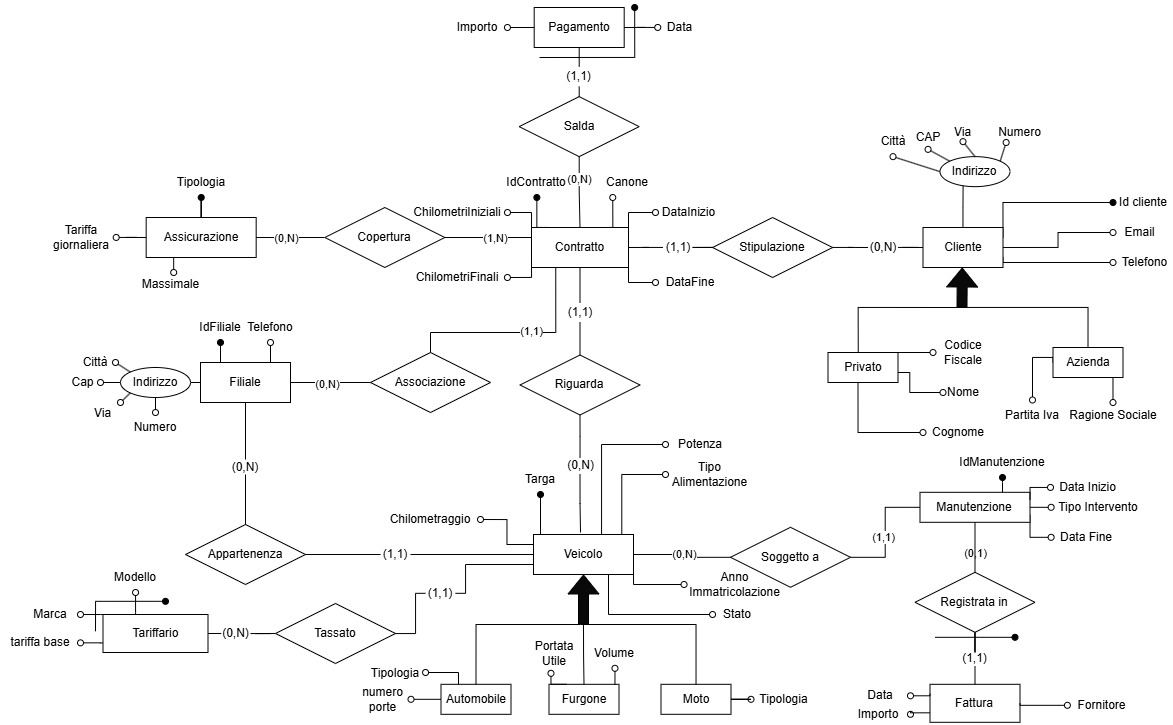
\includegraphics[width=14.65cm]{Modello_Concettuale.jpg} % Modifica la larghezza e il percorso
    \caption{\textit{Diagramma Entità-Relazione del database per il Noleggio Auto}} 
\end{figure}

\section{Progettazione concettuale}

Dalla Figura~\ref{fig:er}, che mostra il diagramma Entità-Relazionale \textit{(E-R)} abbiamo la rappresentazione di ciò che viene descritto in sezione \ref{analisirequisiti}.


\subsection{Vincoli non rappresentabili in schema ER}
Lo schema \ref{fig:er} non permette di rappresentare i seguenti vincoli:
\begin{itemize}
    \item Uno stesso veicolo non può essere associato a due contratti i cui intervalli temporali si sovrappongono.
\end{itemize}
\begin{itemize}
    \item Un veicolo in manutenzione non può essere noleggiato.
\end{itemize}
\begin{itemize}
    \item La somma di tutti i pagamenti riferiti ad un contratto non deve superare il canone totale. 
\end{itemize}


% ******************** GESTIONE TABELLE*************************
% **************************************************************
% **************************************************************
% **************************************************************
% **************************************************************


\begin{table}[H] \label{TabellaSchemaEr}
\centering
\begin{tabularx}{\textwidth}{|>{\centering\arraybackslash}4|
                                >{\centering\arraybackslash}X|
                                >{\centering\arraybackslash}X|
                                >{\centering\arraybackslash}X|}
\hline
\textbf{Entità} & \textbf{Descrizione} & \textbf{Attributi} & \textbf{Identificatore} \\
\hline
Contratto & Contratto di noleggio & IdContratto, Canone, DataInizio, DataFine, ChilometriIniziali, ChilometriFinali & IdContratto \\
\hline
Cliente & Individuo con un contratto di noleggio & IdCliente, Email, Telefono, Città, Cap, Via, Numero & IdCliente \\
\hline
Privato & Cliente che agisce in proprio & CF, Nome, Cognome & \quad \\
\hline
Azienda & Cliente che agisce per conto di un'azienda & Partita Iva, Ragione & \quad \\
\hline
Veicolo & Veicolo con stato variabile & Targa, Chilometraggio, Potenza, Tipo Alimentazione, Anno Immatricolazione, Stato & Targa \\
\hline
Automobile & Autovettura destinata a trasporto di persone & TIpologia, Numero Porte & \quad \\
\hline
Furgone & Veicolo commerciale adibito a trasporto merci & Portata utile, volume & \quad \\
\hline
Moto & Veicolo a due ruote & Tipologia & \quad \\
\hline
Filiale & Filiale di noleggio autorizzata & IdFiliale, Telefono, Città, Cap, Via, Numero & IdFiliale \\
\hline
Assicurazione & Copertura applicabile ad un veicolo, RCA obbligatorio & Tipologia, Tariffa giornaliera, Massimale & Tipologia \\
\hline
Manutenzione & Manutenzione ordinaria o straordinaria di un veicolo & IdManutenzione, Datainizio, DataFine, TipoIntervento & IdManutenzione \\
\hline
Fattura & Fattura di tracciamento per una manutenzione & Fornitore, data, importo & Relazione "Registrata in" \\
\hline
Pagamento & Pagamento tracciato relativo ad un contratto & DataPagamento, importo & Data, Relazione "Salda" \\
\hline
Tariffario & Contiene tariffe base dei vari modelli di veicolo & Modello, Marca, Tariffa Base & Marca, Modello \\
\hline
\end{tabularx}
\end{table}

\begin{table}[H]
\centering
\begin{tabularx}{\textwidth}{|>{\centering\arraybackslash}4|
                                >{\centering\arraybackslash}X|
                                >{\centering\arraybackslash}X|
                                >{\centering\arraybackslash}2|}
\hline
\textbf{Relazione} & \textbf{Descrizione} & \textbf{Componente} & \textbf{Attributi} \\
\hline
Salda & pagamento Salda una parte/o tutto il contratto & Contratto, Pagamento & \\
\hline
Stipulazione & Stipulazione di un contratto & Contratto, Cliente& \\
\hline
Riguarda & Il veicolo noleggiato a cui fa riferimento il contratto & Contratto, Veicolo& \\
\hline
Copertura & Le coperture assicurative che coprono il veicolo del contratto & Contratto, Assicurazione& \\
\hline
Associazione & La filiale dove il contratto è stato sottoscritto e dove avviene il ritiro e la consegna del veicolo noleggiato & Contratto, Filiale& \\
\hline
Appartenenza & Filiale fisica di appartenenza del veicolo & Filiale, Veicolo& \\
\hline
Soggetto a & manutenzioni ordinarie o straordinarie & Veicolo, Manutenzione& \\
\hline
Tassato a & tariffa applicata in base al modello e marca & Veicolo, Tariffario& \\
\hline
Registrata in  & Certificazione manutenzione con una fattura fiscale & Manutenzione, Fattura& \\
\hline

\end{tabularx}
\end{table}


\section{Progettazione Logica}

\subsection{Analisi delle ridondanze}
Assumendo i seguenti volumi nella base di dati:

\begin{table}[H]
\centering
\begin{tabular}{|l|c|l|}
\hline
\textbf{Concetto} & \textbf{Costrutto} & \textbf{Volume}\\
\hline
Contratto & E & 10000 \\
\hline
Riguarda & R & 10000\\
\hline
Veicolo & E & 250\\
\hline
Soggetto a & R & 1000\\
\hline
Tariffario & E & 125\\
\hline
Tassato & R & 250\\
\hline
Assicurazione & E & 8\\
\hline
Copertura & R & 15000\\
\hline
\end{tabular}
\end{table}
%\newpage

% Gestione delle RIDONDANZE

\noindent
L’attributo \textbf{Stato} in \textbf{Veicolo}, che memorizza lo stato attuale del veicolo (disponibile, in manutenzione, in noleggiato), presenta ridondanza.\\
Questo può essere infatti ottenuto verificando se esiste un contratto attivo “oggi” per quel veicolo (datainizio<= oggi <= datafine in Contratto) oppure se esiste una manutenzione attiva “oggi” (in Manutenzione).\\
Questo attributo viene modificato ad ogni inizio/fine contratto e manutenzione e viene visualizzato ad ogni nuovo noleggio:

\begin{itemize}
\item \textbf{Operazione 1} (50 volte al giorno): Verifica disponibilità veicolo prima di stipulare un contratto (lettura di stato)
\item \textbf{Operazione 2} (50 volte al giorno): Inizio Noleggio (memorizza un nuovo contratto, che modifica lo stato del veicolo -> Noleggiato)
\item \textbf{Operazione 3} (50 volte al giorno): Fine Noleggio (chiusura contratto, modifica lo stato del veicolo -> Disponibile)
\item \textbf{Operazione 4} (2 volte al giorno): Inizio manutenzione (memorizza una nuova manutenzione del veicolo, modifica lo stato -> in Manutenzione)
\item \textbf{Operazione 5} (2 volte al giorno): Fine Manutenzione (modifica lo stato -> Disponibile)
\end{itemize}

\noindent
La seguente analisi serve per stabilire se sia utile o meno tenere l’attributo ridondante
STATO in VEICOLO.\\
%RIDONDANZA STATO
\textbf{CON RIDONDANZA} Analizziamo prima il costo totale con ridondanza:\\
\textbf{Operazione 1}:
\begin{table} [h!]
\centering
\begin{tabular}{|p{2cm}|p{2cm}|p{2cm}|p{2cm}|p{1.5cm}|}
\hline
\textbf{Concetto} & \textbf{Costrutto} & \textbf{Accessi} & \textbf{Tipo} & \textbf{Volume} \\
\hline
Veicolo & E & 1 & Lettura & x50 \\
\hline
\end{tabular}
\end{table}
\\
\textbf{Operazione 2}:
\begin{table} [h!]
\centering
\begin{tabular}{|p{2cm}|p{2cm}|p{2cm}|p{2cm}|p{1.5cm}|}
\hline
\textbf{Concetto} & \textbf{Costrutto} & \textbf{Accessi} & \textbf{Tipo} & \textbf{Volume} \\
\hline
Contratto & E & 1 & Scrittura & x50 \\
\hline
Riguarda & R & 1 & Scrittura & x50 \\
\hline
Veicolo & E & 1 & Scrittura & x50 \\
\hline
\end{tabular}
\end{table}
\\
\textbf{Operazione 3}:
\begin{table} [h!]
\centering
\begin{tabular}{|p{2cm}|p{2cm}|p{2cm}|p{2cm}|p{1.5cm}|}
\hline
\textbf{Concetto} & \textbf{Costrutto} & \textbf{Accessi} & \textbf{Tipo} & \textbf{Volume} \\
\hline
Riguarda & R & 1 & Lettura & x50 \\
\hline
Veicolo & E & 1 & Scrittura & x50 \\
\hline
\end{tabular}
\end{table}
\\
\textbf{Operazione 4}:
\begin{table} [H]
\centering
\begin{tabular}{|p{2cm}|p{2cm}|p{2cm}|p{2cm}|p{1.5cm}|}
\hline
\textbf{Concetto} & \textbf{Costrutto} & \textbf{Accessi} & \textbf{Tipo} & \textbf{Volume} \\
\hline
Manutenzione & E & 1 & Scrittura & x2 \\
\hline
Soggetto a & R & 1 & Scrittura & x2 \\
\hline
Veicolo & E & 1 & Scrittura & x2 \\
\hline
\end{tabular}
\end{table}

\noindent
\textbf{Operazione 5}:
\begin{table} [H]
\centering
\begin{tabular}{|p{2cm}|p{2cm}|p{2cm}|p{2cm}|p{1.5cm}|}
\hline
\textbf{Concetto} & \textbf{Costrutto} & \textbf{Accessi} & \textbf{Tipo} & \textbf{Volume} \\
\hline
Soggetto a & R & 1 & Lettura & x2 \\
\hline
Veicolo & E & 1 & Scrittura & x2 \\
\hline
\end{tabular}
\end{table}
\noindent
Assumendo costo doppio per gli accessi in scrittura:\\
Costo Totale: $50\cdot10 + 2\cdot9 = 519$
\\
\noindent
% gestione senza ridondanza per attributo STATO
\textbf{SENZA RIDONDANZA} Analizziamo il costo totale senza ridondanza.


\noindent
\textbf{Operazione 1}:
\begin{table} [h!]
\centering
\begin{tabular}{|p{2cm}|p{2cm}|p{2cm}|p{2cm}|p{1.5cm}|}
\hline
\textbf{Concetto} & \textbf{Costrutto} & \textbf{Accessi} & \textbf{Tipo} & \textbf{Volume} \\
\hline
Riguarda & R & 1 & Lettura & x50 \\
\hline
Contratto & E & 40 & Lettura & x50 \\
\hline
Soggetto A & R & 1 & Lettura & x50 \\
\hline
Manutenzione & E & 4 & Lettura & x50 \\
\hline
\end{tabular}
\end{table}

\noindent
\textit{Nota}(calcolo degli accessi):\\
Poiché un veicolo ha in media 40 contratti (10000 /250 = 40) senza ridondanza dobbiamo controllare ogni contratto del veicolo per stabilire se nessuno è attivo in questo momento.\\
\noindent
\textbf{Operazione 2}:
\begin{table} [h!]
\centering
\begin{tabular}{|p{2cm}|p{2cm}|p{2cm}|p{2cm}|p{1.5cm}|}
\hline
\textbf{Concetto} & \textbf{Costrutto} & \textbf{Accessi} & \textbf{Tipo} & \textbf{Volume} \\
\hline
Contratto & E & 1 & Scrittura & x 50 \\
\hline
Riguarda & R & 1 & Lettura & x 50 \\
\hline
\end{tabular}
\end{table}

\noindent
\textbf{Operazione 3}: Nessun accesso dovuto a questa operazione
\\\\
\noindent
\textbf{Operazione 4}:
\begin{table} [H]
\centering
\begin{tabular}{|p{2cm}|p{2cm}|p{2cm}|p{2cm}|p{1.5cm}|}
\hline
\textbf{Concetto} & \textbf{Costrutto} & \textbf{Accessi} & \textbf{Tipo} & \textbf{Volume} \\
\hline
Manutenzione & E & 1 & Scrittura & x 2 \\
\hline
Soggetto a & R & 1 & Scrittura & x 2 \\
\hline
\end{tabular}
\end{table}

\noindent
\textbf{Operazione 5}: Nessun accesso dovuto a questa operazione\\

\noindent
Assumendo costo doppio per gli accessi in scrittura:\\
 Costo Totale: $50 + 50\cdot40 + 50 + 50\cdot4 + 50\cdot4 + 2\cdot4 = 2508$


\noindent
A seguito dell’analisi è stato deciso di mantenere la ridondanza \textbf{stato} per ottimizzare gli accessi.\\

%\newpage



\noindent
L’attributo \textbf{Chilometraggio} in \textbf{Veicolo} è ridondante: esso infatti è derivabile da chilometri finali in Contratto, dell’ultimo contratto effettuato per quel veicolo.\\
Questo attributo viene modificato ad ogni fine contratto, e viene visualizzato per definire i chilometri iniziali su un nuovo contratto. \\
(I volumi che usiamo per dati sono quelli già definiti precedentemente)


\begin{itemize}
\item \textbf{Operazione 1} (50 volte al giorno): Lettura chilometraggio per stipulazione nuovo contratto;
\item \textbf{Operazione 2} (50 volte al giorno): Fine noleggio: aggiornamento chilometri finali;
\end{itemize}

\noindent
la seguente analisi serve per stabilire se sia utile o meno tenere l’attributo ridondante \\CHILOMETRAGGIO in VEICOLO.\\
\noindent
\textbf{CON RIDONDANZA} Analizziamo prima il costo totale con ridondanza:\\
\textbf{Operazione 1}:\\
\begin{table} [h!]
\centering
\begin{tabular}{|p{2cm}|p{2cm}|p{2cm}|p{2cm}|p{1.5cm}|}
\hline
\textbf{Concetto} & \textbf{Costrutto} & \textbf{Accessi} & \textbf{Tipo} & \textbf{Volume} \\
\hline
Veicolo & E & 1 & Lettura & x50 \\
\hline
\end{tabular}
\end{table}
\\
\textbf{Operazione 2}:\\
\begin{table} [h!]
\centering
\begin{tabular}{|p{2cm}|p{2cm}|p{2cm}|p{2cm}|p{1.5cm}|}
\hline
\textbf{Concetto} & \textbf{Costrutto} & \textbf{Accessi} & \textbf{Tipo} & \textbf{Volume} \\
\hline
Contratto & E & 1 & Lettura & x50 \\
\hline
Riguarda & R & 1 & Lettura & x50 \\
\hline
Veicolo & E & 1 & Scrittura & x50 \\
\hline
\end{tabular}
\end{table}
\\

\noindent
Assumendo costo doppio per gli accessi in scrittura:\\
Costo Totale: $50 + 50 + 50 + 50\cdot2 = 250$
\\

\noindent
\textbf{SENZA RIDONDANZA} Analizziamo il costo totale senza ridondanza.\\

\noindent
\textbf{Operazione 1}:
\begin{table} [h!]
\centering
\begin{tabular}{|p{2cm}|p{2cm}|p{2cm}|p{2cm}|p{1.5cm}|}
\hline
\textbf{Concetto} & \textbf{Costrutto} & \textbf{Accessi} & \textbf{Tipo} & \textbf{Volume} \\
\hline
Riguarda & R & 1 & Lettura & x50 \\
\hline
Contratto & E & 40 & Lettura & x50 \\
\hline
\end{tabular}
\end{table}

\noindent
\textbf{Operazione 2 }: Nessun accesso dovuto a questa operazione\\


\noindent
Assumendo costo doppio per gli accessi in scrittura:\\
 Costo Totale: $50 + 50\cdot40 = 2050$


\noindent
Anche in questo caso, a seguito dell’analisi è stato deciso di mantenere la ridondanza\\ \textbf{Chilometraggio} per ottimizzare gli accessi\\

%\newpage

\noindent
L’attributo \textbf{Canone} in \textbf{Contratto}, che memorizza il canone del contratto  presenta ridondanza.\\
Questo può essere infatti ottenuto calcolando la somma delle varie Tariffe Giornaliere scelte per quel contratto sommate alla tariffa del veicolo che si intende noleggiare il tutto moltiplicato per la durata del contratto;\\
Questo attributo viene scritto ad ogni nuovo contratto e viene visualizzato per controllo saldo pagamenti.

\begin{itemize}
\item \textbf{Operazione 1} (50 volte al giorno): Creazione di un contratto (calcolo canone);
\item \textbf{Operazione 2} (150 volte al giorno): Lettura canone per controllo saldo pagamenti;
\end{itemize}

\noindent
la seguente analisi serve per stabilire se sia utile o meno tenere l’attributo ridondante \\CANONE in CONTRATTO.\\

\textbf{CON RIDONDANZA} Analizziamo prima il costo totale con ridondanza:\\

\textbf{Operazione 1}:\\
\begin{table} [h!]
\centering
\begin{tabular}{|p{2cm}|p{2cm}|p{2cm}|p{2cm}|p{1.5cm}|}
\hline
\textbf{Concetto} & \textbf{Costrutto} & \textbf{Accessi} & \textbf{Tipo} & \textbf{Volume} \\
\hline
Copertura & R & 1 & Lettura & x50 \\
\hline
Assicurazione & E & 2 & Lettura & x50 \\
\hline
Riguarda & R & 1 & Lettura & x50 \\
\hline
Veicolo & E & 1 & Lettura & x50 \\
\hline
Tassato & R & 1 & Lettura & x50 \\
\hline
Tariffario & E & 1 & Lettura & x50 \\
\hline
Contratto & E & 1 & Lettura & x50 \\
\hline
Contratto & E & 1 & Scrittura & x50 \\
\hline
\end{tabular}
\end{table}
\\

\noindent
\textit{Nota}(calcolo degli accessi in Assicurazione):\\
Assumendo due assicurazioni scelte in media per ogni ceontratto. \\

\textbf{Operazione 2}:\\
\begin{table} [h!]
\centering
\begin{tabular}{|p{2cm}|p{2cm}|p{2cm}|p{2cm}|p{1.5cm}|}
\hline
\textbf{Concetto} & \textbf{Costrutto} & \textbf{Accessi} & \textbf{Tipo} & \textbf{Volume} \\
\hline
Contratto & E & 1 & Scrittura & x150 \\
\hline
\end{tabular}
\end{table}
\\

\noindent
Assumendo costo doppio per gli accessi in scrittura:\\
Costo Totale: $50\cdot6 + 50\cdot2 + 50\cdot2 +150 = 650$


\textbf{SENZA RIDONDANZA} Analizziamo il costo totale senza ridondanza.\\

\noindent
\textbf{Operazione 1 }: Nessun accesso dovuto a questa operazione\\
%\newpage
\noindent
\textbf{Operazione 2}:\\
\begin{table} [h!]
\centering
\begin{tabular}{|p{2cm}|p{2cm}|p{2cm}|p{2cm}|p{1.5cm}|}
\hline
\textbf{Concetto} & \textbf{Costrutto} & \textbf{Accessi} & \textbf{Tipo} & \textbf{Volume} \\
\hline
Contratto & E & 1 & Lettura & x150 \\
\hline
Copertura & R & 1 & Lettura & x150 \\
\hline
Assicurazione & E & 2 & Lettura & x150 \\
\hline
Riguarda & R & 1 & Lettura & x150 \\
\hline
Veicolo & E & 1 & Lettura & x150 \\
\hline
Tassato & R & 1 & Lettura & x150 \\
\hline
Tariffario & E & 1 & Lettura & x150 \\
\hline
\end{tabular}
\end{table}
\\
\noindent
Assumendo costo doppio per gli accessi in scrittura:\\
 Costo Totale: $150\cdot8 = 1200$\\

\noindent
Anche in questo caso, a seguito dell’analisi è stato deciso di mantenere la ridondanza \textbf{Canone} per ottimizzare gli accessi.\\

%Eliminazioni delle generalizzazioni

\subsection{Eliminazione delle generalizzazioni}
Nello schema concettuale realizzato, le generalizzazioni adottate sono di tipo \textit{esclusivo e totale}: ogni entità figlia specializza l'entità padre senza sovrapposizioni, e tutte le istanze dell'entità padre appartengono necessariamente a una delle sottoclassi.
\noindent
Queste generalizzazioni vengono eliminate attraverso una ristrutturazione dello schema concettuale, con l'obiettivo di semplificare l'implementazione del modello relazionale.\\
\noindent
Per entrambe le generalizzazioni si è adottata l'opzione di sostituzione con relationship che prevede il mantenimento dell'entità padre collegata a ciascuna entità figlia introducendo delle relazioni tra di loro.\\
L'opzione di accorpamento nel padre è stata scartata perché avrebbe introdotto molti valori nulli, poiché ogni entità figlia presenta attributi specifici.\\
L'opzione di accorpamento dei figli invece è stata scartata perché avrebbe eliminato l'entità padre, obbligando le entità collegate (come Contratto con Cliente e Manutenzione con Veicolo) a mantenere più chiavi esterne nullable.
\noindent
L'eliminazione della generalizzazione \textbf{Veicolo}, introduce le relazioni Is-Automobile, Is-Furgone e Is-Moto,  utilizzando come chiave esterna la targa del veicolo per collegare le entità "figlie" a Veicolo.\\
L'entità Veicolo mantiene gli attributi comuni a tutte le tipologie di mezzi e mantiene la targa come identificatore univoco, garantendo un unico punto di riferimento a tutte le entità che referenziano un veicolo.\\
Le Entità figlie contengono esclusivamente gli attributi specifici della relativa categoria di veicolo.
\noindent
In modo analogo l'eliminazione della generalizzazione \textbf{Cliente} introduce le relazioni Is-Privato e Is-Azienda, utilizzando come chiave esterna l'identificatore univoco per collegare le entità Privato e Azienda a Cliente.

%\newpage

\subsubsection{Schema E-R ristrutturato}
\begin{figure}[h!] \label{SchemaER-Ristrutturato}
    \centering
    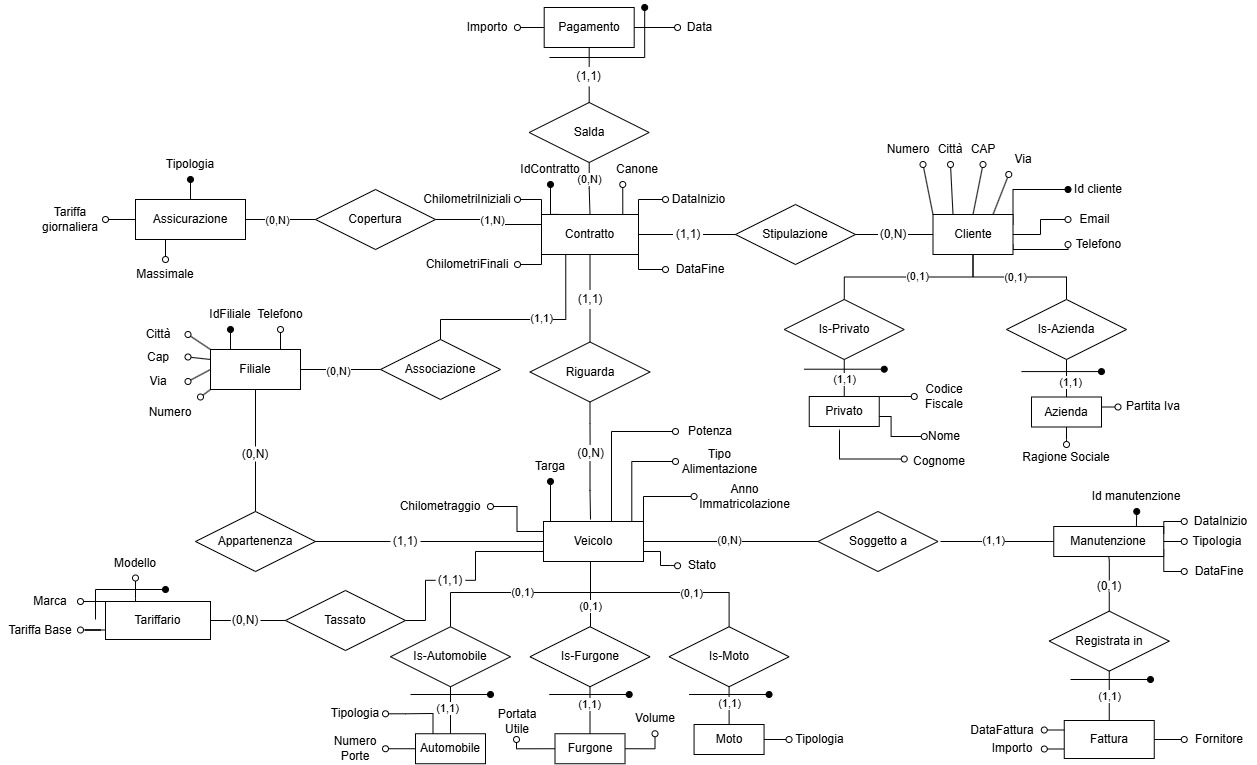
\includegraphics[width=14.5cm]{Modello_logico.jpg} 
    \caption{\textit{Diagramma E-R modificato del database per il Noleggio Auto}} 
\end{figure}
\noindent
Nelle successive sezioni vengono indicate le procedure che spiegano le modifiche che hanno portato allo schema ristrutturato di Figura~\ref{SchemaER-Ristrutturato}.

\subsection{Schema relazionale}
\label{SchemaRelazionale}
Lo schema ristrutturato presente nella sezione \ref{SchemaER-Ristrutturato} rappresenta lo \textbf{schema logico} in forma grafica. Di seguito abbiamo un elenco di tutte le tabelle derivate dallo schema logico (La presenza di * vicino ad un attributo indica che è nullable):
\begin{itemize}
    \item \textbf{Filiale}(\underline{IdFiliale}, Telefono, Città, Via, Numero, CAP)
    \item \textbf{IdCliente}(\underline{Cliente}, Email, Telefono, Città, Via, Numero, CAP)
    \item \textbf{Tariffario}(\underline{Marca, Modello}, TariffaBase)
    \item \textbf{Veicolo}(\underline{Targa}, Chilometraggio, AnnoImmatricolazione, Potenza, TipoAlimentazione, Stato, TariffarioMarca, TariffarioModello, Filiale)
    \\
    - Veicolo.(TariffarioMarca, TariffarioModello) $\rightarrow$ Tariffario(Marca,Modello)
    \\
    - Veicolo.Filiale $\rightarrow$ Filiale.IdFiliale
    \item \textbf{Automobile}(\underline{Veicolo}, Tipologia, NumeroPorte)
    \\
    - Automobile.Veicolo $\rightarrow$ Veicolo.Targa
    \item \textbf{Furgone}(\underline{Veicolo}, Volume, PortataUtile)
    \\
    - Furgone.Veicolo $\rightarrow$ Veicolo.Targa
    \item \textbf{Moto}(\underline{Veicolo}, Tipologia)
    \\
    - Moto.Veicolo $\rightarrow$ Veicolo.Targa
    \item \textbf{Contratto}(\underline{IdContratto}, ChilometriIniziali, Canone, DataInizio, DataFine, ChilometriFinali*, Veicolo, Cliente, Filiale)
    \\
    - Contratto.Veicolo $\rightarrow$ Veicolo.Targa
    \\
    - Contratto.Cliente $\rightarrow$ Cliente.IdCliente
    \\
    - Contratto.Filiale $\rightarrow$ Filiale.IdFiliale
    \item \textbf{Pagamento}(\underline{Contratto, DataPagamento}, Importo)
    \\
    - Pagamento.Contratto $\rightarrow$ Contratto.IdContratto
    \item \textbf{Assicurazione}(\underline{Tipologia}, TariffaGiornaliera, Massimale)
    \item \textbf{Copertura}(\underline{Assicurazione, Contratto})
    \\
    - Copertura.Assicurazione $\rightarrow$ Assicurazione.Tipologia
    \\
    - Copertura.Contratto $\rightarrow$ Contratto.IdContratto
    \item \textbf{Manutenzione}(\underline{IdManutenzione}, DataInizio, DataFine*, Tipologia, Veicolo)
    \\
    - Manutenzione.Veicolo $\rightarrow$ Veicolo.Targa
    \item \textbf{Fattura}(\underline{Manutenzione}, Fornitore, DataFattura, Importo)
    \\
    - Fattura.Manutenzione $\rightarrow$ Manutenzione.IdManutenzione
    \item \textbf{Privato}(\underline{IdCliente}, CodiceFiscale, Nome, Cognome)
    \\
    - Privato.IdCliente $\rightarrow$ Cliente.IdCliente
    \item \textbf{Azienda}(\underline{IdCliente}, PartitaIva, RagioneSociale)
    \\
    - Azienda.IdCliente $\rightarrow$ Cliente.IdCliente
    
\end{itemize}

\section{Implementazione PostgreSQL e Query}
Il file \textit{noleggioauto.sql} contiene il codice SQL usato per la \textbf{generazione} delle tabelle, la \textbf{creazione} dei type, il loro \textbf{popolamento} e il codice per la \textbf{definizione} delle query utilizzate. Inoltre è presente l'istruzione di creazione di un indice per ottimizzare la quarta query.

\subsection{Definizioni delle query}
\textbf{Query 1}: Mostrare i contratti che risultano avere canone non saldato e il loro saldo rimanente.
\begin{lstlisting}
SELECT C.idContratto, C.canone as SaldoRimanente
FROM contratto C LEFT JOIN Pagamento P ON C.idcontratto = P.contratto
GROUP BY C.idcontratto, C.canone
HAVING sum(P.importo) IS NULL
UNION
SELECT C.idContratto, ( C.canone - sum(P.importo)) as SaldoRimanente
FROM contratto C JOIN Pagamento P ON C.idcontratto = P.contratto
GROUP BY C.idcontratto, C.canone
having sum(P.importo) < C.canone
order by idcontratto;
\end{lstlisting}
\begin{figure}[H]
    \centering
    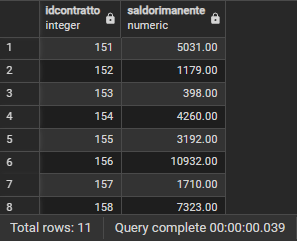
\includegraphics[width=0.3\linewidth]{Query1.png}
\end{figure}
\noindent
\textbf{Query 2}: Mostrare i clienti che hanno noleggiato almeno un auto di lusso e la somma dei canoni dei contratti a loro associati
\begin{lstlisting}
CREATE VIEW sommacanonecliente as
SELECT cl.idcliente, SUM(co.canone) as sommacanone
FROM contratto co join cliente cl on co.cliente = cl.idcliente
group by cl.idcliente
order by cl.idcliente;

SELECT DISTINCT scc.idcliente, scc.sommacanone
FROM sommacanonecliente scc join contratto con on scc.idcliente = con.cliente
join veicolo v on v.targa = con.veicolo
join tariffario t on v.tariffariomarca = t.marca and v.tariffariomodello = t.modello
where t.tariffabase > 200
order by scc.idcliente
\end{lstlisting}
\begin{figure}[h!]
    \centering
    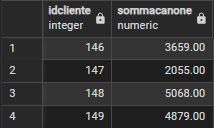
\includegraphics[width=0.3\linewidth]{Query2.png}
\end{figure}
\noindent
\textbf{Query 3}: Mostrare targa, marca, modello e numero di manutenzioni straordinarie dei veicoli che sono stati soggetti ad almeno una manutenzione straordinaria
\begin{lstlisting}
CREATE VIEW contomanutenzioni as
SELECT v.targa, count(*) as nmanutenzioni
FROM veicolo v join manutenzione m on v.targa = m.veicolo
WHERE m.Tipologia = 'STRAORDINARIA'
GROUP BY targa;

SELECT cm.targa, t.marca, t.modello, cm.nmanutenzioni
FROM contomanutenzioni cm join veicolo v on cm.targa = v.targa 
JOIN tariffario t on v.tariffariomarca = t.marca and v.tariffariomodello = t.modello
\end{lstlisting}
\begin{figure}[H]
    \centering
    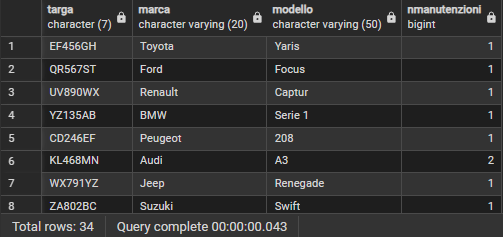
\includegraphics[width=0.5\linewidth]{Query3.png}
\end{figure}

\textbf{Query 4}: Mostrare per la filiale x numero di veicoli totali, disponibili, noleggiati e in manutenzione (x = 1 in questo caso)
\begin{lstlisting}
select F.idfiliale, V.Totali, V1.Disponibili, V2.Noleggiati, V3.Manutenzione
from Filiale F LEFT JOIN (
    select filiale, count(*) as Totali
    from Veicolo
    GROUP BY filiale
) as V on F.idfiliale=V.filiale
LEFT JOIN (
    select filiale, count(*) as Disponibili
    from Veicolo 
    where Stato = 'DISPONIBILE'
    GROUP BY filiale
) as V1 on F.idfiliale=V1.filiale
LEFT JOIN (
    select filiale, count(*) as Noleggiati
    from Veicolo 
    where Stato = 'NOLEGGIATO'
    GROUP BY filiale
) as V2 on F.idfiliale=V2.filiale
LEFT JOIN (
    select filiale, count(*) as Manutenzione
    from Veicolo 
    where Stato = 'MANUTENZIONE'
    GROUP BY filiale
) as V3 on F.idfiliale=V3.filiale
where F.idfiliale = 1
\end{lstlisting}
\begin{figure}[h!]
    \centering
    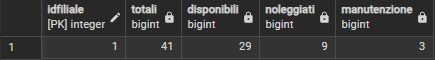
\includegraphics[width=0.5\linewidth]{Query4.png}
\end{figure}
%\newpage
\noindent
\textbf{Query 5}: Mostrare le assicurazioni più sottoscritte nell'anno 2025 (RCA esclusa)
\begin{lstlisting}
CREATE VIEW frequenzaAssicurazione as
select a.Tipologia, COUNT(*) as sottoscrizioni
from contratto con join copertura cop on con.idcontratto = cop.contratto
join assicurazione a on cop.assicurazione = a.tipologia
where con.datainizio >= '2025-01-01' and con.datainizio <= '2025-12-31' 
and a.tipologia <> 'RCA'
group by a.Tipologia;

select fa.tipologia, fa.sottoscrizioni
from frequenzaAssicurazione fa
where fa.sottoscrizioni = (select max(sottoscrizioni) from frequenzaAssicurazione)
\end{lstlisting}
\begin{figure}[h!]
    \centering
    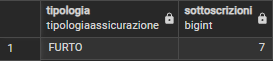
\includegraphics[width=0.4\linewidth]{Query5.png}
\end{figure}





\subsection{Creazione dell' indice}
Per migliorare le performance della \textbf{Query 4} viene introdotto un indice composto B-tree sugli attributi \textit{Filiale}, \textit{Stato} della tabella \textbf{Veicolo}.\\
Abbiamo optato per un Btree, anche se la query da ottimizzare utilizza esclusivamente uguaglianze, poiché PostgreSQL non permette la creazione di hash composti e sebbene si possano fare indici hash separati (uno per Filiale, uno per Stato) l'aggiornamento di due hash distinti porterebbe ad un overhead notevole.
La Query lavora sulla tabella Veicolo, selezionando i veicoli associati a una specifica filiale distinguendoli in base al loro stato.\\
L’attributo Filiale consente di restringere la ricerca dei veicoli appartenenti alla filiale considerata, mentre lo Stato permette di distinguere i veicoli in base al loro stato operativo.
\begin{lstlisting}
CREATE INDEX idx_StatoFiliale_veicolo ON VEICOLO(Filiale, Stato);
\end{lstlisting}
In questo modo il sistema può individuare più velocemente il numero di veicoli appartenenti alla determinata filiale e il loro stato, evitando una scansione completa di tutti i veicoli il cui numero può aumentare nel tempo dovuto alla creazione di nuovi filiali o all'aumento dei clienti che necessitano sempre più veicoli.\\
L’introduzione di questo indice comporta un costo aggiuntivo dovuto alle varie operazioni di aggiornamento, tuttavia tale costo è ritenuto accettabile, poiché la query rappresenta un operazione gestionale frequente per il monitoraggio dei veicoli nelle diverse filiali.



\section{Codice C}
Il file \textit{noleggioauto.c} contiene il codice necessario ad accedere alla base dati, il quale può essere compilato ed eseguito tramite i comandi:
\begin{minted}{bash}
gcc noleggioauto.c -L dependencies \lib -lpq -o noleggioauto
./noleggioauto
\end{minted}   
Appena eseguito, il programma chiederà di accedere al database tramite nome utente e password tramite la funzione \textbf{Authenticate()};
in caso di esito positivo, verrà mostrata la lista delle query disponibili e verrà lasciata all'utente la possibilità di selezionare tramite input da tastiera la query desiderata. \\
Il programma continua l'esecuzione finché l'utente non inserisce 0 come input e digitando 6 si può effettuare nuovamente la stampa delle query disponibili.\\
La query 4 è stata resa \textbf{parametrica} per permettere all'utente di scegliere la filiale da consultare.\\ L'inserimento del valore che determina la query da eseguire e l'inserimento della filiale di riferimento della quarta query hanno un controllo di integrità dell'input di base.
\end{document}